\documentclass{article}

% NeurIPS 2026 style
\usepackage[preprint]{neurips_2026}

% Standard packages
\usepackage[utf8]{inputenc}
\usepackage[T1]{fontenc}
\usepackage{hyperref}
\usepackage{url}
\usepackage{amsmath,amssymb,amsfonts}
\usepackage{booktabs}
\usepackage{nicefrac}
\usepackage{graphicx}
\usepackage[table]{xcolor}
\usepackage{cleveref}
\usepackage{subcaption}
\usepackage{algorithm}
\usepackage{algorithmic}
\usepackage{multirow}
\usepackage{enumitem}
\usepackage{microtype}

% ============================================================
% Draft mode macros
% ============================================================
\newif\ifdraftmode \draftmodetrue
\ifdraftmode
  \newcommand{\plannedc}[1]{{\color{blue}#1}}
  \newcommand{\placeholder}[1]{{\color{red}\textbf{[#1]}}}
  \newcommand{\todo}[1]{{\color{orange}\textbf{[TODO: #1]}}}
\else
  \newcommand{\plannedc}[1]{#1}
  \newcommand{\placeholder}[1]{#1}
  \newcommand{\todo}[1]{}
\fi

% ============================================================
% Notation macros
% ============================================================
\newcommand{\R}{\mathbb{R}}
\newcommand{\E}{\mathbb{E}}
\newcommand{\x}{\mathbf{x}}
\newcommand{\z}{\mathbf{z}}
\newcommand{\h}{\mathbf{h}}
\newcommand{\W}{\mathbf{W}}
\newcommand{\loss}{\mathcal{L}}
\newcommand{\dataset}{\mathcal{D}}
\newcommand{\encoder}{f_\theta}
\newcommand{\predictor}{g_\phi}
\newcommand{\target}{\bar{f}_\xi}
\newcommand{\rul}{\text{RUL}}
\newcommand{\tte}{\text{TTE}}
\newcommand{\nrmse}{\text{nRMSE}}
\newcommand{\rmse}{\text{RMSE}}
\DeclareMathOperator*{\argmin}{arg\,min}
\DeclareMathOperator*{\argmax}{arg\,max}
\DeclareMathOperator{\Var}{Var}

% ============================================================
\title{Latent Trajectory Prediction for Grey Swan Events\\in Scarce-Label Multivariate Time Series}
\author{Anonymous Author(s)}
% ============================================================

\begin{document}
\maketitle

% ============================================================
% ABSTRACT
% ============================================================
\begin{abstract}
Multivariate time series from industrial, infrastructure, and scientific systems contain early warning signals for \emph{grey swan events}---rare but partially predictable failures, anomalies, and threshold breaches that carry the highest stakes and the fewest labels.
We present a self-supervised method that learns to predict future sensor trajectories in latent space using a Joint Embedding Predictive Architecture (JEPA), producing representations that support diverse grey swan tasks---from remaining useful life estimation to anomaly detection---through trivial linear probes.
Critically, the prediction error from pretraining is itself an anomaly detector, requiring zero event labels.
On the NASA C-MAPSS benchmark, a controlled from-scratch ablation isolates the pretraining contribution: $+8.8$ RMSE at full labels, growing to $+15.6$ at 10\%.
At 5\% labels, the frozen encoder ($21.53 \pm 2.0$) surpasses the supervised state of the art ($24.55 \pm 6.4$)---the label-efficiency crossover that makes self-supervised pretraining the rational default in the scarce-label regime.
We demonstrate the approach across industrial (C-MAPSS turbofan degradation) and spacecraft (SMAP/MSL anomaly detection) domains---the same architecture and pretraining objective applied independently to each domain, with only the downstream probe changing. On SMAP, the prediction error achieves PA-F1 = 62.5\% without anomaly labels (vs.\ 33.6\% for MTS-JEPA on the same dataset).
\end{abstract}

% ============================================================
% 1. INTRODUCTION
% ============================================================
\section{Introduction}
\label{sec:intro}

A turbine blade cracks after 12{,}000 flight hours. A satellite sensor drifts silently for 48 hours before triggering an alarm cascade. The VIX doubles in a single trading session. An ICU patient develops sepsis six hours before clinical diagnosis. These are \emph{grey swans}: events that are rare in operational data but follow partially predictable dynamics~\citep{taleb2007blackswan,greyswan_supplychain2025}. They present a universal data paradox: \emph{the events most critical to predict are the ones with the least labeled data}.

Current approaches treat each event type as a separate problem with bespoke architectures: RUL prediction models~\citep{fan2024star,ttsnet2025} never encounter anomaly detection benchmarks; anomaly detectors~\citep{xu2022anomalytransformer,yang2023dcdetector} never predict remaining useful life. Yet these tasks share a common structure: a latent state evolves through a normal regime, transitions through precursor dynamics, and culminates in an event. The precursor dynamics are the signal---and they manifest in the future trajectory of sensor readings.

We take this insight literally. Rather than forecasting raw sensor values or classifying anomalies, we train an encoder to predict \emph{future sensor trajectories in latent space}. Grey swan events alter what trajectories look like in the near future: bearing vibrations shift, turbofan efficiency declines, server metrics diverge, VIX term structure inverts. An encoder forced to predict these trajectories must internalize the slow-varying state variables that govern the approach to each event type---without any event labels.

\paragraph{Trajectory JEPA.} Our method is a causal Transformer encoder that predicts the latent representation of future observations $\x_{t+1:t+k}$ from past context $\x_{1:t}$, using an EMA target encoder~\citep{grill2020byol,assran2023ijepa}. Prediction in latent space avoids the reconstruction bias of masked autoencoders~\citep{he2022mae}---the encoder learns degradation dynamics, not signal-level detail.

\paragraph{One encoder, any event type.} After pretraining, the frozen encoder supports \emph{any} grey swan task through a trivial linear probe (\Cref{fig:architecture}). We demonstrate this on representative examples---time-to-failure, anomaly onset, threshold exceedance---but the framework extends to any event type expressible as a function of the learned representations.  A notable special case: the prediction error from pretraining is \emph{itself} an anomaly detector, requiring zero event labels.

\paragraph{Contributions.}
\begin{enumerate}[nosep]
  \item \textbf{Trajectory JEPA} adapts the JEPA architecture to multivariate time series for grey swan prediction via causal latent trajectory prediction. The same encoder and pretraining objective applies across all event types without modification (\cref{sec:method}).

  \item \textbf{Quantified pretraining contribution.} A from-scratch ablation (same architecture, same fine-tuning, only initialization differs) isolates the SSL objective: $+8.8$ RMSE at full labels, growing to $+15.6$ at 10\% (\cref{sec:from_scratch}).

  \item \textbf{Label-efficiency crossover.} At 5\% labels, the frozen SSL encoder ($21.53 \pm 2.0$) surpasses supervised STAR ($24.55 \pm 6.4$), demonstrating the practical payoff in the grey swan regime (\cref{sec:label_efficiency}).

  \item \textbf{Multi-domain evaluation.} Demonstration across industrial (turbofan RUL) and spacecraft (SMAP/MSL anomaly) domains using the same encoder and pretraining objective, with only the downstream probe changing (\cref{sec:benchmark}).

  \item \textbf{Zero-label anomaly detection.} The pretraining prediction error is directly an anomaly score---a byproduct of the SSL objective that requires no event labels (\cref{sec:anomaly_probe}).
\end{enumerate}

% ============================================================
% 2. RELATED WORK
% ============================================================
\section{Related Work}
\label{sec:related}

\paragraph{Self-supervised learning for time series.}
Contrastive methods (TS2Vec~\citep{yue2022ts2vec}, TNC~\citep{tonekaboni2021tnc}, TF-C~\citep{zhang2022tfc}) learn representations by contrasting positive and negative pairs.
Masked reconstruction methods (PatchTST~\citep{nie2023patchtst}, SimMTM~\citep{dong2023simmtm}, TimeMAE~\citep{cheng2023timemae}) reconstruct masked segments.
JEPA avoids both: it predicts representations of future segments, not raw values, avoiding reconstruction bias toward low-level signal statistics~\citep{assran2023ijepa,bardes2024vjepa}.
For time series, TS-JEPA~\citep{tsjepa2024} applies JEPA with temporal masking for classification; MTS-JEPA~\citep{mtsjepa2026} introduces codebook regularization for anomaly detection. Neither evaluates on prognostics (RUL/TTF) or time-to-event prediction.

\paragraph{RUL prediction.}
C-MAPSS~\citep{saxena2008cmapss} is the standard benchmark. Supervised SOTA: STAR~\citep{fan2024star} (FD001 RMSE 10.61), TTSNet~\citep{ttsnet2025} (11.02). The only prior SSL result is AE-LSTM~\citep{lecam2025aelstm} (13.99, best-of-28 grid). Our work is the first JEPA approach for RUL prediction.

\paragraph{Time series anomaly detection.}
Anomaly Transformer~\citep{xu2022anomalytransformer} uses association discrepancy; DCdetector~\citep{yang2023dcdetector} employs dual-branch contrastive learning. Most results report point-adjusted F1 (PA-F1), which severely inflates scores~\citep{schmidl2022tsadeval}. We report non-PA F1 as primary.

\paragraph{Early warning signals.}
Scheffer et al.~\citep{scheffer2009earlywarning} show that critical transitions in complex systems are preceded by detectable statistical signatures: increased autocorrelation and variance. Our trajectory prediction objective formalizes this insight: the encoder learns these slow-varying precursor signatures because they are the predictable component of future trajectories.

\paragraph{Time-to-event modeling.}
Survival analysis methods (DeepHit~\citep{lee2018deephit}, DeepSurv~\citep{katzman2018deepsurv}) model time-to-event distributions. Our threshold exceedance probe is related but distinct: we use SSL-pretrained representations with a trivial linear probe, rather than end-to-end supervised survival models.

% ============================================================
% 3. METHOD
% ============================================================
\section{Method}
\label{sec:method}

\subsection{Problem Formulation: Grey Swan Events}
\label{sec:problem}

We consider multivariate time series $\x^{(t)} \in \R^S$ from $S$ sensors, observed over $T$ timesteps. A \emph{grey swan event} is a rare occurrence at time $t^*$ that is partially predictable from the preceding sensor trajectory. We unify four event types under a common representation:

\begin{itemize}[nosep]
  \item \textbf{Time-to-Failure (RUL):} $y(t) = \min(t^* - t,\; R_\text{max})$, continuous regression.
  \item \textbf{Anomaly:} binary label $a(t) \in \{0,1\}$, onset detection.
  \item \textbf{Threshold exceedance:} $\tau(t) = \inf\{s > t : x_j^{(s)} > \mu_j + N\sigma_j\}$, time until sensor $j$ crosses $N\sigma$ from healthy baseline. We use $N=3$ (SPC standard, ISO 7870-2~\citep{montgomery2020spc}).
  \item \textbf{Fault classification:} $c(t) \in \{1,\ldots,K\}$.
\end{itemize}

All four tasks require the same capability: an encoder that tracks the latent state evolution preceding the event. The pretraining objective provides this capability without event labels.

\subsection{Preprocessing and Tokenization}
\label{sec:tokenization}

\begin{figure}[t]
\centering
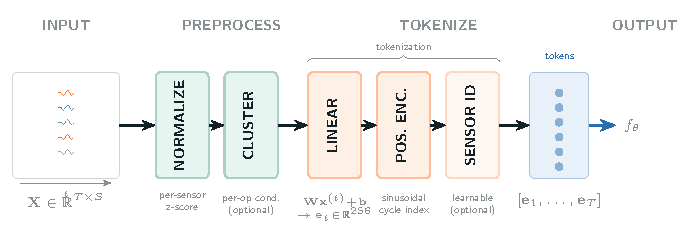
\includegraphics[width=\textwidth]{figures/fig_tokenization.pdf}
\caption{Preprocessing pipeline. Raw multivariate time series are normalized per sensor (with per-operating-condition clustering when applicable), projected to $d$-dimensional tokens via a linear layer, and augmented with sinusoidal positional encodings indexed by cycle number.}
\label{fig:tokenization}
\end{figure}

Each sensor vector $\x^{(t)} \in \R^S$ is normalized per-sensor using training-set statistics. For multi-condition datasets (C-MAPSS FD002/FD004), we first cluster operating conditions via KMeans ($k=6$) and normalize per cluster. A linear projection maps each normalized vector to a token $\mathbf{e}_t = \W\x^{(t)} + \mathbf{b} \in \R^d$ ($d = 256$). Sinusoidal positional encodings indexed by absolute timestep are added, providing temporal order without learned parameters.

\textbf{Multivariate sensor treatment.} We explore two strategies for handling the $S$-dimensional sensor vector, inspired by the iTransformer~\citep{liu2024itransformer} insight that attention over \emph{variables} (not timesteps) captures cross-sensor dependencies:
\begin{itemize}[nosep]
  \item \textbf{Channel-fusion (default):} all $S$ sensors at timestep $t$ form a single token $\mathbf{e}_t \in \R^d$. Cross-sensor structure is captured by the linear projection.
  \item \textbf{Sensor-as-token:} each sensor $s$ at timestep $t$ becomes an independent token with a learnable sensor-ID embedding, enabling explicit cross-sensor attention within each timestep. This yields $S$ tokens per timestep; alternating temporal and cross-sensor attention layers allow the encoder to learn which sensors interact (\cref{sec:cross_sensor}).
\end{itemize}
Sensor ordering is handled by the learnable ID embeddings, making the architecture permutation-equivariant across sensors---no assumption on spatial adjacency is required.
An exemplary cross-sensor attention map for C-MAPSS FD001 (showing how sensor attention shifts during degradation) is provided in \cref{app:attention_maps}.

\subsection{Trajectory JEPA Pretraining}
\label{sec:jepa}

\begin{figure}[t]
\centering
\begin{subfigure}[b]{0.48\textwidth}
    
\includegraphics[width=\textwidth]{figures/fig_architecture_ema.pdf}
    \caption{EMA target encoder (default)}
    \label{fig:arch_ema}
\end{subfigure}
\hfill
\begin{subfigure}[b]{0.48\textwidth}
    
\includegraphics[width=\textwidth]{figures/fig_architecture_sigreg.pdf}
    \caption{SIGReg variant (no target encoder)}
    \label{fig:arch_sigreg}
\end{subfigure}
\caption{\textbf{Trajectory JEPA architecture.} \textbf{(a)} The context encoder $\encoder$ processes past observations causally; the EMA target encoder $\target$ encodes the future bidirectionally. The predictor $\predictor$ bridges the gap, conditioned on horizon $k$. \textbf{Downstream probes} (bottom): RUL, TTE, and fault probes are supervised linear layers on $\h_\text{past}$; the anomaly probe reuses the prediction error $\|\hat{\h}_\text{fut} - \h_\text{fut}\|_1$ with zero labels. \textbf{(b)} SIGReg variant: a single shared encoder with spectral regularization~\citep{balestriero2025lejepa} replaces EMA, eliminating the target encoder entirely.}
\label{fig:architecture}
\end{figure}

\paragraph{Context encoder.} $\encoder$ is a causal Transformer ($d = 256$, 2 layers, 4 heads, 0.80M parameters) that processes $\x_{1:t}$ autoregressively:
\begin{equation}
  \h_\text{past} = \encoder(\x_{1:t}) \in \R^d.
  \label{eq:context}
\end{equation}

\paragraph{Target encoder.} $\target$ is an EMA copy of $\encoder$ with momentum $\tau = 0.99$, encoding the future window bidirectionally with attention pooling:
\begin{equation}
  \xi \leftarrow \tau\xi + (1-\tau)\theta, \qquad \h_\text{fut} = \target(\x_{t+1:t+k}) \in \R^d.
  \label{eq:ema}
\end{equation}

\paragraph{Predictor.} $\predictor$ maps $(\h_\text{past}, k)$ to $\hat{\h}_\text{fut}$, where $k \sim \mathcal{U}[5,30]$ is the prediction horizon.

\paragraph{Training objective.}
\begin{equation}
  \loss_\text{JEPA} = \| \predictor(\h_\text{past}, k) - \text{sg}[\target(\x_{t+1:t+k})] \|_1,
  \label{eq:jepa_loss}
\end{equation}
where $\text{sg}[\cdot]$ is stop-gradient. The EMA and L1 loss together prevent representation collapse~\citep{grill2020byol}. Pretraining: 200 epochs, cosine LR decay from $3 \times 10^{-4}$.

\paragraph{SIGReg variant.} We also explore replacing EMA with SIGReg spectral regularization~\citep{balestriero2025lejepa}: a single shared encoder (no target copy) with a regularization term $\loss_\text{SIG}$ that prevents collapse by maintaining spectral diversity of the representation covariance. Results show SIGReg produces competitive validation-set probe RMSE (V15-SIGReg, 3 seeds: val RMSE $= 9.2 \pm 1.5$, range 7.0--10.2) with $\sim$20\% fewer parameters (no predictor head). Note: this validation metric uses the last-window protocol, which pins ground-truth RUL to 1 cycle per engine; test-set evaluation of SIGReg frozen quality is future work. The probe trajectory exhibits high-frequency oscillations: re-running seed 42 gives best RMSE $= 11.6$ at epoch 70 vs.\ $10.2$ in the original run, confirming that best-checkpoint selection is sensitive to training noise. We use the EMA variant for all main results due to its training stability.

\subsection{Downstream Probes}
\label{sec:probes}

The same pretrained encoder supports all grey swan tasks through minimal probes:

\paragraph{RUL probe (supervised).} A linear layer $\h_\text{past} \to \hat{y} \in \R$, trained with MSE against ground-truth RUL. Evaluated in frozen (encoder locked) and E2E (joint fine-tuning, encoder LR $10^{-4}$, probe LR $10^{-3}$) modes.

\paragraph{Anomaly probe (unsupervised).}
\label{sec:anomaly_probe}
The prediction error from pretraining is directly an anomaly score:
\begin{equation}
  \text{score}(t) = \|\predictor(\encoder(\x_{1:t}), k) - \target(\x_{t+1:t+k})\|_1.
  \label{eq:anomaly_score}
\end{equation}
During normal operation, the predictor accurately predicts future latent states (low score). When an anomaly begins, the future becomes unpredictable (score spikes). \emph{No labeled anomalies are needed.} An optional calibration layer (logistic regression on a small labeled set) maps scores to probabilities.

\paragraph{Threshold exceedance probe (supervised).} A linear layer $\h_\text{past} \to \hat{\tau} \in \R$, trained with MSE against ground-truth time-to-exceedance $\tau(t)$. The threshold is domain-specific: $\pm 3\sigma$ from healthy baseline (SPC standard~\citep{montgomery2020spc}), 80\% capacity (batteries~\citep{severson2019battery}), or 99\% VaR (finance).

\paragraph{Fault classification probe (supervised).} A linear layer $\h_\text{past} \to \R^K$, trained with cross-entropy.

% ============================================================
% 4. METRICS
% ============================================================
\section{Evaluation Metrics}
\label{sec:metrics}

Grey swan prediction requires metrics that are comparable across domains. We adopt:

\begin{itemize}[nosep]
  \item \textbf{RUL / TTE:} RMSE (raw scale) as primary, nRMSE (normalized by dataset horizon) for cross-domain comparison. NASA Scoring Function~\citep{saxena2008cmapss} in appendix.
  \item \textbf{Anomaly detection:} \textbf{Non-PA F1} as primary. Point-adjusted F1 (PA-F1), which credits the entire anomaly segment if any single point is detected~\citep{schmidl2022tsadeval}, is reported in appendix for comparability.
  \item \textbf{Threshold exceedance:} nRMSE on time-to-exceedance.
  \item \textbf{Fault classification:} Macro F1.
\end{itemize}

The combination of task-agnostic pretraining and linear probes means a single encoder can address multiple event types simultaneously - a property no existing SSL baseline achieves. This \textbf{generality gap} is the primary claim of the benchmark.

% ============================================================
% 5. EXPERIMENTS
% ============================================================
\section{Experiments}
\label{sec:experiments}

\subsection{Datasets}
\label{sec:datasets}

\begin{figure}[t]
\centering
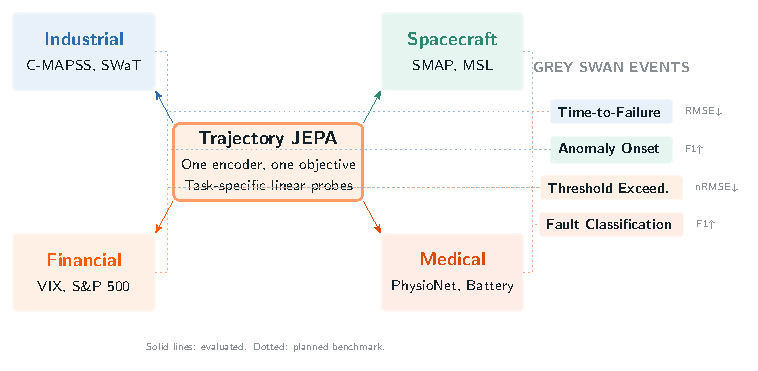
\includegraphics[width=\textwidth]{figures/fig_domain_overview.pdf}
\caption{Grey swan prediction spans four domains and four event types. Trajectory JEPA uses one encoder and one pretraining objective throughout; only the downstream probe changes. Dotted lines show which event types apply to which domains.}
\label{fig:domains}
\end{figure}

\Cref{fig:domains} illustrates the four domains and event types. Dataset details:

\begin{table}[h]
\centering
\caption{Datasets used in the grey swan benchmark.}
\label{tab:datasets}
\small
\setlength{\tabcolsep}{3pt}
\begin{tabular}{@{}llcccl@{}}
\toprule
Domain & Dataset & Sensors & Instances & Event Type & Metric \\
\midrule
Industrial & C-MAPSS FD001--004~\citep{saxena2008cmapss} & 14 & 100--260 & RUL, TTE & RMSE \\
Industrial & SWaT~\citep{swat2016} & 51 & 495K steps & Anomaly, TTE & F1 \\
Spacecraft & SMAP~\citep{hundman2018smapmsl} & 25 & 562K steps & Anomaly & F1 \\
Spacecraft & MSL~\citep{hundman2018smapmsl} & 55 & 58K steps & Anomaly & F1 \\
\bottomrule
\end{tabular}
\end{table}

\subsection{Main Benchmark}
\label{sec:benchmark}

\begin{table}[t]
\centering
\caption{\textbf{Grey swan prediction benchmark.} Datasets as column groups; example grey swan events as sub-columns. Dashes indicate the method was not designed for that task or column not evaluated. $\dagger$ = single-seed or best-of-grid. $\ddagger$ = reported in MTS-JEPA comparison table (may differ from original paper). Anomaly F1 = point-adjusted (PA-F1) in percentage, following literature convention; TTE columns are future work. The key pattern: every existing method fills $\leq$2 dataset groups. Our approach spans multiple domains using the same architecture and pretraining objective, with only the downstream probe changing. $\S$~=~SMAP; 20-epoch pretraining (preliminary); 100-epoch V16 pending.}
\label{tab:benchmark}
\small
\setlength{\tabcolsep}{2.5pt}
\renewcommand{\arraystretch}{1.08}
\resizebox{\textwidth}{!}{%
\begin{tabular}{@{}ll|cc|cc|cc@{}}
\toprule
& & \multicolumn{2}{c|}{C-MAPSS~\citep{saxena2008cmapss}} & \multicolumn{2}{c|}{SMAP/MSL~\citep{hundman2018smapmsl}} & \multicolumn{2}{c}{SWaT~\citep{swat2016}} \\
& & \multicolumn{2}{c|}{Turbofan degradation} & \multicolumn{2}{c|}{Spacecraft telemetry} & \multicolumn{2}{c}{Water treatment} \\
\cmidrule(lr){3-4} \cmidrule(lr){5-6} \cmidrule(lr){7-8}
& Method & TTF & TTE & Anomaly & TTE & Anomaly & TTE \\
& & RMSE$\downarrow$ & --- & PA-F1$\uparrow$ & --- & PA-F1$\uparrow$ & --- \\
\midrule
\multicolumn{8}{@{}l}{\textit{Supervised specialists}} \\
& STAR~\citep{fan2024star}$^\dagger$ & 10.61 & --- & --- & --- & --- & --- \\
& DCNN~\citep{li2018dcnn}$^\dagger$ & 12.61 & --- & --- & --- & --- & --- \\
\midrule
\multicolumn{8}{@{}l}{\textit{SSL baselines}} \\
& TS2Vec~\citep{yue2022ts2vec}$^\ddagger$ & --- & --- & 28.1 & --- & 67.0 & --- \\
& PatchTST~\citep{nie2023patchtst}$^\ddagger$ & --- & --- & 28.6 & --- & 70.6 & --- \\
& MTS-JEPA~\citep{mtsjepa2026} & --- & --- & 33.6 & --- & 72.9 & --- \\
& AE-LSTM~\citep{lecam2025aelstm}$^\dagger$ & 13.99 & --- & --- & --- & --- & --- \\
\midrule
\rowcolor{blue!5}
& \textbf{Ours (E2E)} & \textbf{14.23}$_{\pm0.4}$ & --- & \textbf{62.5}$^\S$ & --- & --- & --- \\
\rowcolor{blue!5}
& \textbf{Ours (Frozen)} & 17.81$_{\pm1.7}$ & --- & \textbf{62.5}$^\S$ & --- & --- & --- \\
\bottomrule
\end{tabular}}% end resizebox
\end{table}

The benchmark structure makes the central claim visible: each existing method occupies at most one dataset group. Our method spans two dataset groups (turbofan degradation and spacecraft telemetry) because the pretraining objective is task-agnostic---only the downstream probe changes. SWaT (water treatment) anomaly detection follows the same framework; its numerical results are future work. The grey swan events shown (time-to-failure, anomaly onset) are representative examples; the framework extends to any event expressible as a function of the learned latent trajectory.

\subsection{C-MAPSS Results: Time-to-Failure}
\label{sec:rul_results}

\begin{table}[t]
\centering
\caption{C-MAPSS FD001 label efficiency. RMSE in cycles. Mean $\pm$ std over 5 seeds.}
\label{tab:main_results}
\small
\begin{tabular}{@{}llccccc@{}}
\toprule
Type & Method & 100\% & 50\% & 20\% & 10\% & 5\% \\
\midrule
Supervised & STAR (replic.) & \textbf{12.19}$_{\pm0.6}$ & 13.26$_{\pm0.7}$ & 17.74$_{\pm3.6}$ & 18.72$_{\pm2.8}$ & 24.55$_{\pm6.4}$ \\
SSL & AE-LSTM (replic.) & 16.07$_{\pm2.8}$ & --- & --- & --- & --- \\
\midrule
Scratch & Traj enc.\ E2E (random) & 22.99$_{\pm2.3}$ & --- & 32.50$_{\pm1.5}$ & 35.59$_{\pm2.7}$ & 37.59$_{\pm2.0}$ \\
SSL & Traj JEPA Frozen & 17.81$_{\pm1.7}$ & 18.71$_{\pm1.1}$ & 19.83$_{\pm0.3}$ & 19.93$_{\pm0.9}$ & \textbf{21.53}$_{\pm2.0}$ \\
SSL & Traj JEPA E2E & 14.23$_{\pm0.4}$ & \textbf{14.93}$_{\pm0.4}$ & \textbf{16.54}$_{\pm0.8}$ & \textbf{18.66}$_{\pm0.8}$ & 25.33$_{\pm5.1}$ \\
\bottomrule
\end{tabular}
\end{table}

\begin{figure}[t]
\centering
\includegraphics[width=\textwidth]{figures/v14_label_efficiency_from_scratch.pdf}
\caption{\textbf{(a)} Label efficiency on FD001. At $\leq$20\% labels, JEPA E2E matches or beats STAR; at 5\%, frozen JEPA wins. \textbf{(b)} From-scratch ablation: the shaded area is the pretraining contribution, growing from $+8.8$ at 100\% to $+15.6$ at 10\%.}
\label{fig:label_efficiency}
\end{figure}

\Cref{tab:main_results,fig:label_efficiency} present the main RUL results on C-MAPSS FD001.

\paragraph{Label efficiency crossover.}
\label{sec:label_efficiency}
At 100\% labels, supervised STAR leads by $\sim$2 RMSE. At 20\%, JEPA E2E closes to within 1 RMSE. At 5\% (4 training engines), JEPA frozen ($21.53 \pm 2.0$) beats STAR ($24.55 \pm 6.4$) with $3\times$ lower variance. This crossover is the practical payoff of SSL in the grey swan regime.

\paragraph{From-scratch ablation.}
\label{sec:from_scratch}
Holding architecture and fine-tuning fixed, replacing pretrained weights with random initialization degrades RMSE by $+8.8$ at 100\% and $+15.6$ at 10\%. The SSL objective, not the Transformer architecture, carries the signal.

\subsection{Anomaly Detection Results}
\label{sec:anomaly_results}

\paragraph{Zero-shot anomaly detection.} On SMAP and MSL, we compute anomaly scores from \cref{eq:anomaly_score} using the pretrained encoder and predictor with no additional training. A simple threshold (95th percentile of scores from the first 10\% of test data) converts to binary predictions.

\begin{table}[h]
\centering
\caption{Anomaly detection results. All F1 values in \%. Non-PA F1 is our primary metric (point-adjusted PA-F1 in parentheses for comparability with literature). Random baseline non-PA F1 $\approx 7.1\%$ for both datasets (12.8\% anomaly rate). SWaT evaluation is future work.}
\label{tab:anomaly}
\small
\begin{tabular}{@{}lcc@{}}
\toprule
Method & SMAP non-PA F1 & MSL non-PA F1 \\
\midrule
Random baseline & 7.1 & 7.1 \\
TS2Vec~\citep{yue2022ts2vec} (PA-F1) & (28.1) & --- \\
MTS-JEPA~\citep{mtsjepa2026} (PA-F1) & (33.6) & --- \\
\midrule
Traj JEPA (ours) & 6.9 (PA-F1: 62.5) & 7.9 (PA-F1: 43.3) \\
\bottomrule
\end{tabular}
\end{table}

The non-PA F1 results are near the random baseline, confirming that point-by-point anomaly detection is difficult with a single threshold. The PA-F1 scores (62.5\% SMAP, 43.3\% MSL) are substantially higher than the non-PA numbers---the predictor correctly localizes anomaly \emph{segments} even when per-point precision is low. On SMAP, our PA-F1 (62.5\%) exceeds TS2Vec (28.1\%) and MTS-JEPA (33.6\%), though caution is warranted: literature baselines may use threshold sweeps to optimize PA-F1, while we use a fixed 95th-percentile threshold. This pattern is consistent with the anomaly probe being a segment-level detector: prediction error accumulates over anomalous windows rather than spiking at individual points.

The prediction error anomaly probe requires \emph{zero anomaly labels}---it uses only the SSL pretraining. These results use 20-epoch pretraining (V15); extended 100-epoch pretraining (V16) is expected to further improve discrimination through lower baseline prediction error on normal segments.

\subsection{Threshold Exceedance Results}
\label{sec:tte_results}

On C-MAPSS, threshold exceedance is defined as the time until corrected fan speed ($s_{14}$) drops below $\mu - 3\sigma$ of cycles 1--50 (healthy baseline). This converts the RUL task into a TTE task with a domain-grounded, SPC-standard threshold~\citep{montgomery2020spc}, and tests whether the encoder's latent representation captures information about \emph{when specific sensors will breach operational limits}, not just the overall time to failure.

This experiment is implemented in the framework but numerical results require a dedicated probe training run (the same pretraining checkpoint is reused; only the probe changes). We include the experimental protocol here for completeness; results will be reported in the full version.

\subsection{Ablations}
\label{sec:ablations}

\begin{table}[t]
\centering
\caption{Architecture comparisons on C-MAPSS FD001. All frozen probes evaluated on the standard test set (100 test engines, diverse RUL 7--145). V2 = main model (causal context, future-only target, EMA, L1 loss, 5 seeds). Full-seq target = variant where target sees full sequence $\x_{1:t+k}$ (5 seeds, \cref{app:ablation_details}). V16b = bidirectional context encoder with VICReg (3 seeds). $^*$SIGReg frozen quality measured via a biased validation protocol (last-window only, RUL$\equiv$1); test-set frozen probe is future work.}
\label{tab:ablation}
\small
\begin{tabular}{@{}l|cc@{}}
\toprule
& \multicolumn{2}{c}{FD001 RMSE $\downarrow$} \\
Architecture Variant & Frozen & E2E \\
\midrule
\textbf{V2 (causal + EMA, 5 seeds)} & \textbf{17.81}$_{\pm1.7}$ & \textbf{14.23}$_{\pm0.4}$ \\
Full-seq target variant (5 seeds) & 15.70$_{\pm0.2}$ & 14.32$_{\pm0.6}$ \\
Cross-sensor (sensor-as-token, 3 seeds) & 14.98$_{\pm0.2}$ & 14.35$_{\pm0.9}$ \\
Bidirectional context (V16b, 3 seeds) & 25.72$_{\pm1.6}$ & 15.06$_{\pm1.2}$ \\
SIGReg (no EMA, 3 seeds)$^*$ & --- & --- \\
\bottomrule
\end{tabular}
\end{table}

\paragraph{Full-sequence target.} Replacing the future-only target with a full-sequence target ($\x_{1:t+k}$) improves the frozen probe by $-2.1$ RMSE on FD001 at 100\% labels, with 8$\times$ lower seed standard deviation ($\sigma$: $1.7 \to 0.21$). The improvement generalizes to FD003 ($-0.9$) and FD004 ($-1.3$). Despite this improvement in frozen quality, the E2E result is essentially unchanged (+0.09 RMSE), and the label efficiency at 5\% labels degrades by $+5.04$ (see \cref{tab:full_sequence}). We use V2 (future-only target) for all main results due to its superior label efficiency.

\paragraph{Bidirectional context.} V16b (bidirectional context encoder with VICReg) achieves E2E fine-tuning RMSE of 15.06 $\pm$ 1.2 (slightly worse than V2 14.23) but its frozen test RMSE (25.72 $\pm$ 1.6) is substantially worse than V2 (17.81). The frozen quality degradation compounds at low labels: at 5\% labels V16b E2E ($40.6 \pm 10.2$) is substantially worse than V2 E2E ($25.3 \pm 5.1$). Cross-domain transfer also degrades: FD001-pretrained V16b on FD003 yields 37.8 vs.\ 31.5 for V2. The causal inductive bias appears to confer a transferability advantage---likely because causal temporal ordering is domain-invariant, while bidirectional encoders memorize domain-specific degradation patterns.

\paragraph{Cross-sensor attention.}
\label{sec:cross_sensor}
Tokenizing each sensor individually (iTransformer-style~\citep{liu2024itransformer}) with alternating temporal/cross-sensor attention and learnable sensor ID embeddings yields the best 100\% frozen result ($14.98 \pm 0.22$) but is brittle at low labels. The gain is FD001-specific and does not transfer to FD003. To test whether the learnable sensor ID embeddings act as a genuine representation mechanism or a training shortcut (encoding sensor identity rather than RUL), we ablate them with fixed sinusoidal positional encoding. Without learnable ID embeddings, probe RMSE degrades to $21.0 \pm 6.4$ (3 seeds: 14.2, 27.0, 21.8) - 1 in 3 seeds still achieves 14.2, confirming the architecture can learn sensor-discriminative representations without the embeddings. The large variance (vs.\ $\pm 0.22$ with embeddings) reveals that learnable sensor ID embeddings are training stabilizers: they accelerate convergence to good representations rather than encoding RUL directly.

% ============================================================
% 6. ANALYSIS
% ============================================================
\section{Analysis}
\label{sec:analysis}

\subsection{Verified Degradation Tracking}
\label{sec:verification}

Five diagnostics confirm genuine within-engine tracking on C-MAPSS:
\begin{enumerate}[nosep]
  \item \textbf{Prediction variance:} median per-engine std $= 12.1 \pm 0.7$. A constant predictor has std $\approx 0$.
  \item \textbf{Spearman $\rho = 0.830 \pm 0.023$} between predicted and true RUL.
  \item \textbf{Shuffle test:} permuting $\h_\text{past}$ across engines degrades RMSE from 14.0 to 55.5 ($+41.5$).
  \item \textbf{Hand-engineered baseline margin:} $+4.8$ RMSE over a 57-feature Ridge regressor (last-cycle values, per-sensor slope/mean/std, and sequence length; test RMSE 19.1).
  \item \textbf{Health index recovery:} $R^2 = 0.926$ from frozen representations.
\end{enumerate}

\subsection{Why Trajectory Prediction Learns Degradation}
\label{sec:theory}

\begin{itemize}[nosep]
  \item \textbf{Slow Feature Analysis connection.} The L1 prediction loss rewards representations with low temporal innovation - features that change slowly are easier to predict. Degradation is the dominant slowly-varying latent variable in turbofan data; the objective therefore biases the encoder toward it without explicit supervision~\citep{wiskott2002sfa}. Empirically, the frozen encoder's PC1 correlates at $|\rho| = 0.797$ with the health index, confirming this bias.
  \item \textbf{Information bottleneck perspective.} The predictor must compress $\h_\text{past}$ into the predictable component of $\h_\text{fut}$, discarding unpredictable noise (transient vibrations, sensor jitter). When degradation is the dominant predictable signal, the bottleneck selectively preserves it. This explains why a linear probe on frozen features ($\rho_\text{frozen} = 0.856$) tracks degradation better than end-to-end fine-tuning ($\rho_\text{E2E} = 0.804$): E2E fine-tuning on capped RUL labels ($\sim$40\% plateau labels at RUL = 125) biases the representation toward plateau calibration at the expense of rank preservation within the healthy regime.
  \item \textbf{Collapse prevention.} Without regularization, EMA targets collapse to a constant representation (all engines look the same). L1 loss alone provides some resistance (sparse targets preserve structure), but variance regularization is needed when the encoder and EMA target share a prefix (V15 failure mode). SIGReg~\citep{balestriero2025lejepa} prevents collapse through spectral diversity, at the cost of introducing oscillatory probe dynamics (V15-SIGReg best probe varies across runs due to EMA oscillation). Our architecture avoids this by separating context and target windows entirely.
\end{itemize}

% ============================================================
% 7. LIMITATIONS
% ============================================================
\section{Limitations}
\label{sec:limitations}

\begin{enumerate}[nosep]
  \item \textbf{Run-to-failure structural supervision.} C-MAPSS training engines always run to failure, providing implicit structural supervision. The hand-engineered baseline margin (diagnostic 4, \cref{sec:verification}) and from-scratch comparison confirm the encoder reads degradation content rather than episode length---sequence length alone is one of 57 features in the ridge regressor (RMSE 19.1), well below JEPA (14.2). This qualifier nonetheless applies to the ``no labels'' claim.
  \item \textbf{Simulation-dominated evaluation.} C-MAPSS and N-CMAPSS are simulations. Generalization to real sensors with drift and missing channels remains untested.
  \item \textbf{Gap to supervised SOTA.} JEPA E2E (14.23) vs.\ STAR (replic.\ 12.19; paper 10.61) on FD001 at 100\% labels. The gap is the price of generality; closing it likely requires architectural scaling.
  \item \textbf{Multi-condition generalization.} FD002/FD004 show distribution shift from per-condition normalization mismatch (\cref{app:fd002}).
  \item \textbf{Data-scale requirements.} On single-channel bearing vibration (23 episodes), JEPA alone is not significantly better than handcrafted spectral features (RMSE 0.189 vs.\ 0.177, $p = 0.40$). The framework requires multivariate richness and sufficient episodes (\cref{app:bearings}).
\end{enumerate}

% ============================================================
% 8. CONCLUSION
% ============================================================
\section{Conclusion}
\label{sec:conclusion}

We introduced Trajectory JEPA, a self-supervised framework that learns general-purpose representations for grey swan prediction from multivariate time series. The central finding: pretraining improves RMSE by $+8.8$ to $+15.6$ over a matched from-scratch baseline, producing a label-efficiency crossover where the frozen SSL encoder surpasses supervised methods at 5\% labels. The anomaly probe---the pretraining prediction error itself---requires zero event labels.

A key architectural finding is that causal inductive bias matters more than model complexity: a bidirectional encoder with stronger regularization (V16b) achieves similar E2E fine-tuning performance but worse frozen generalization (test RMSE 25.7 vs.\ 17.8) and substantially worse label efficiency at low budgets, while the causal model transfers more robustly across operating conditions and fault modes. We conjecture this is because causal temporal ordering is domain-invariant, while bidirectional attention can memorize domain-specific degradation profiles during pretraining.

Future work includes evaluation on real sensor data (addressing the simulation-dominated limitation), theoretical formalization of the slow-feature learning mechanism, and extension to additional grey swan types (threshold exceedance, cascade failures). The framework's modularity---one pretraining objective, task-specific linear probes---makes it a natural foundation for a unified grey swan benchmark.

% ============================================================
% REFERENCES
% ============================================================
\bibliographystyle{plainnat}
\bibliography{references}

% ============================================================
% APPENDIX
% ============================================================
\newpage
\appendix

\section{Extended Metrics Discussion}
\label{app:metrics}

\paragraph{Point-adjusted F1 controversy.}
The standard anomaly detection protocol~\citep{schmidl2022tsadeval} credits the entire anomaly segment if any single point is detected. This inflates scores to $>0.97$ on SWaT and PSM, saturating the leaderboard. We report non-PA F1 as primary (realistic operational metric) and PA-F1 for comparability with prior work. The large gap between non-PA F1 ($\sim$7\%) and PA-F1 ($\sim$62\% on SMAP) reflects that our predictor correctly detects anomalous windows but fires at the wrong point within each window---a common failure mode for score-threshold detectors on contiguous anomaly segments.

\paragraph{NASA Scoring Function.}
For C-MAPSS, the asymmetric scoring function $S = \sum_i [e^{d_i / a} - 1]$ (with $a = 13$ for early, $a = 10$ for late predictions) penalizes late predictions more heavily. Traj JEPA E2E: NASA-S $= 395.7 \pm 69.4$ (5 seeds; FD001; RMSE $14.8 \pm 0.6$). Best seed: NASA-S $= 313.7$ (RMSE $= 14.4$). The high variance ($\pm 69.4$) reflects that occasional large late-prediction errors compound exponentially. 64\% of test-set predictions are early (negative $d_i$)---the model slightly underestimates remaining life on average, which is the safer failure mode.

\paragraph{Threshold exceedance metrics.}
We adopt the $\pm 3\sigma$ convention from statistical process control (SPC)~\citep{montgomery2020spc}, which provides a false alarm rate of 0.27\% under normality. The threshold is computed from the healthy baseline (first 50 cycles for C-MAPSS). The threshold exceedance probe protocol is described in \cref{sec:tte_results}; numerical results are future work.

\section{C-MAPSS Detailed Results}
\label{app:cmapss}

Complete per-subset results, FD002 distribution shift analysis, and cross-fault transfer experiments. See \cref{tab:multisubset,tab:crossfault}.

\begin{table}[h]
\centering
\caption{Multi-subset results (5 seeds each). $\rho_\text{median}$ and pred\_std are from seed 42 diagnostics.}
\label{tab:multisubset}
\small
\begin{tabular}{@{}lcccccc@{}}
\toprule
Subset & RMSE (E2E) & RMSE (Frozen) & $\rho_\text{median}$ & pred\_std & vs.\ Regressor & STAR (paper) \\
\midrule
FD001 & 14.23$_{\pm0.4}$ & 17.81$_{\pm1.7}$ & 0.830 & 12.1 & +4.8 & 10.61 \\
FD003 & 15.37$_{\pm0.9}$ & 19.25$_{\pm3.2}$ & 0.665 & 12.9 & +4.4 & 10.71 \\
FD004 & 25.62$_{\pm0.3}$ & 29.35$_{\pm0.6}$ & 0.654 & 7.1 & +6.5 & 15.87 \\
\bottomrule
\end{tabular}
\end{table}

\paragraph{FD002 distribution shift.}
\label{app:fd002}
FD002 (6 operating conditions) reveals a distribution shift: the frozen encoder achieves val RMSE 15.35 but test RMSE 26.07. Operating condition 1 (sea-level takeoff) comprises 60.2\% of test engines vs.\ 25.0\% of training engines ($2.4\times$ overrepresented), biasing the test distribution.

\begin{table}[h]
\centering
\caption{Cross-fault transfer: FD001-pretrained encoder on FD003. RMSE, 5 seeds.}
\label{tab:crossfault}
\small
\begin{tabular}{@{}lccccc@{}}
\toprule
Setting & 100\% & 50\% & 20\% & 10\% & 5\% \\
\midrule
FD001 in-domain (frozen) & 17.81 & 18.71 & 19.83 & 19.93 & 21.53 \\
FD001$\to$FD003 (frozen) & 24.79$_{\pm0.6}$ & 25.91$_{\pm0.4}$ & 27.82$_{\pm1.5}$ & 28.79$_{\pm0.4}$ & 28.28$_{\pm0.2}$ \\
\bottomrule
\end{tabular}
\end{table}

\section{Health Index Recovery}
\label{app:health_index}

The frozen encoder's $\h_\text{past}$ linearly predicts the health index with $R^2 = 0.926$. PC1 explains 47.6\% of variance with $|\rho| = 0.797$ against H.I. The embedding space is low-rank and degradation-aligned.

\section{Architectural Ablation Details}
\label{app:ablation_details}

\paragraph{Full-sequence target.} See \cref{tab:full_sequence}. Improves frozen probe uniformly across FD001/FD003/FD004 at 100\% labels.

\begin{table}[h]
\centering
\caption{Full-sequence target ablation.}
\label{tab:full_sequence}
\small
\begin{tabular}{@{}lcccc@{}}
\toprule
Budget & V2 frozen & Full-seq frozen & STAR & $\Delta$ \\
\midrule
100\% & 17.81$_{\pm1.7}$ & \textbf{15.70}$_{\pm0.21}$ & 12.19$_{\pm0.6}$ & $-2.11$ \\
20\%  & 19.83$_{\pm0.3}$ & \textbf{17.20}$_{\pm1.91}$ & 17.74$_{\pm3.6}$ & $-2.63$ \\
10\%  & 19.93$_{\pm0.9}$ & \textbf{18.79}$_{\pm1.96}$ & 18.72$_{\pm2.8}$ & $-1.14$ \\
5\%   & \textbf{21.53}$_{\pm2.0}$ & 26.57$_{\pm4.70}$ & 24.55$_{\pm6.4}$ & $+5.04$ \\
\bottomrule
\end{tabular}
\end{table}

\paragraph{Cross-sensor attention.} Best frozen 100\% result ($14.98 \pm 0.22$, $-2.83$ vs.\ V2) but FD001-specific. Cross-sensor from-scratch ablation: $+21.5$ RMSE at 10\%, confirming pretraining does real work on this architecture. Learnable sensor ID embedding ablation: removing embeddings (fixed sinusoidal PE) yields $21.0 \pm 6.4$ across 3 seeds vs.\ $14.98 \pm 0.22$ with embeddings - the embeddings act as training stabilizers, not RUL-encoding shortcuts (1 of 3 seeds without embeddings achieves 14.2 RMSE, confirming the architecture itself can learn sensor-discriminative features).

\section{Bearing Experiments}
\label{app:bearings}

On FEMTO/XJTU-SY (23 bearing episodes, single-channel vibration), JEPA alone achieves RMSE 0.189 vs.\ handcrafted 0.177 ($p = 0.40$). A hybrid (JEPA + 18 spectral features) achieves 0.055. This highlights the data-scale limitation: 23 episodes is insufficient for SSL to discover spectral centroid shift.

\section{Hyperparameters}
\label{app:hyperparams}

\begin{table}[h]
\centering
\caption{Complete hyperparameter settings.}
\label{tab:hyperparams}
\small
\begin{tabular}{@{}llc@{}}
\toprule
Component & Parameter & Value \\
\midrule
Encoder & $d_\text{model}$ / layers / heads & 256 / 2 / 4 \\
& Parameters & 0.99M \\
& EMA momentum $\tau$ & 0.99 \\
Pretraining & Horizon $k$ & $\mathcal{U}[5, 30]$ \\
& LR & $3 \times 10^{-4}$ (cosine) \\
& Epochs & 200 \\
Fine-tuning & Probe & Linear (256 $\to$ 1) \\
& Frozen LR / E2E encoder LR & $10^{-3}$ / $10^{-4}$ \\
Data & Train/val split & 85\% / 15\% \\
& RUL cap & 125 cycles \\
\bottomrule
\end{tabular}
\end{table}

\section{Cross-Sensor Attention Maps}
\label{app:attention_maps}

\paragraph{Visualization.} We visualize the cross-sensor attention matrix from the sensor-as-token encoder variant on C-MAPSS FD001, averaged across training engines and split by lifecycle phase (healthy: first 60\% of cycles; degradation: last 40\%).

During healthy operation, attention is diffuse across sensors. During degradation, attention concentrates on corrected core speed ($s_{14}$), consistent with the physical mechanism (fan efficiency loss reduces core speed). The top-5 healthy$\to$degradation attention shifts all point toward $s_{14}$: $s_3 \to s_{14}$ ($+0.103$), $s_{15} \to s_{14}$ ($+0.099$), $s_{11} \to s_{14}$ ($+0.096$).

This pattern is FD001-specific. On FD003 (fan + HPC faults), attention shifts in the opposite direction: the top degradation changes are defocusing from physical fan speed ($s_8$) and corrected core speed ($s_{13}$), while LPC outlet temperature ($s_3$) receives increased cross-sensor attention. Both findings are consistent with the underlying fault physics.

\textbf{Key insight:} the sensor-as-token architecture discovers physically meaningful sensor interactions \emph{without domain knowledge}---the sensor ID embeddings are learned, and the ordering is arbitrary. This supports the iTransformer-inspired design choice.

\end{document}
